\documentclass[uplatex,dvipdfmx,a4paper,11pt]{jsarticle}

\usepackage{url}
\usepackage[dvipdfmx]{hyperref}

\usepackage[top=25mm,bottom=25mm,left=25mm,right=25mm]{geometry}

\usepackage{array}
\usepackage{tabularx}
\usepackage{booktabs}
\usepackage{enumitem}
\usepackage{graphicx}
\usepackage{longtable}
\usepackage{listings}

\lstset{
  basicstyle=\ttfamily\scriptsize,
  breaklines=true,
  frame=single,
  numbers=left,
  numberstyle=\tiny,
  tabsize=2,
  showstringspaces=false
}

\setlength{\parindent}{0pt}
\setlength{\parskip}{0.6em}

\usepackage{titlesec}
\titleformat{\section}
  {\normalfont\Large\bfseries}{\thesection.}{0.6em}{}
\titleformat{\subsection}
  {\normalfont\large\bfseries}{\thesubsection}{0.6em}{}
\titlespacing*{\section}{0pt}{1.2em}{0.6em}
\titlespacing*{\subsection}{0pt}{1.0em}{0.4em}

\newcommand{\sectionrule}{\par\medskip\noindent\rule{\linewidth}{0.6pt}\par\medskip}

\renewcommand{\labelitemi}{\textbullet}
\renewcommand{\labelitemii}{\textopenbullet}
\setlist[itemize]{leftmargin=1.6em,itemsep=0.1em,topsep=0.2em}
\setlist[enumerate]{leftmargin=2.0em,itemsep=0.1em,topsep=0.2em}

\providecommand{\textopenbullet}{\ensuremath{\circ}}


\begin{document}


{\LARGE\bfseries 作業ログ}\par\bigskip

報告者：佐藤涼菜

報告日：7月8日

プロジェクト名：マジカル☆観覧車

\sectionrule


\section{進捗サマリー（要約）}

\begin{itemize}
  \item 全体進捗率：100[％]
  \item マイルストーン達成状況：テストフェーズの結合テストを継続実施
  \item 主要成果：
    \begin{itemize}
      \item {結合テスト（No.3121, 3141, 3211, 3212）を継続実施}
    \end{itemize}
  \item 重大課題（影響度：高）：
    \begin{itemize}
      \item {特になし}
    \end{itemize}
\end{itemize}

\sectionrule


\section{作業ログ（詳細トラッキング）}

\subsection{作業ログ}

\renewcommand{\arraystretch}{1.2}

\small

\begin{longtable}{|c|p{2.2cm}|c|c|c|c|p{2.4cm}|p{3.1cm}|}
\caption{作業ログ} \\
\hline
No. & 作業項目 & 開始日 & 予定完了日 & 状態 & 進捗率 & 依存関係・ブロッカー & コメント \\
\hline
\endfirsthead

\hline
No. & 作業項目 & 開始日 & 予定完了日 & 状態 & 進捗率 & 依存関係・ブロッカー & コメント \\
\hline
\endhead

\hline
\multicolumn{8}{r}{次ページへ続く} \\
\hline
\endfoot

\hline
\endlastfoot

3121 &
演奏開始の合図送信確認 &
6/10 &
7/7 &
完了 &
100\% &
無 &
グループで集まり実施．\\
\hline

3141 &
レーザー受信確認 &
6/17 &
7/7 &
完了 &
100\% &
無 &
グループで集まり実施．\\
\hline

3211 &
開始信号の受信確認 &
6/10 &
7/7 &
完了 &
100\% &
無 &
グループで集まり実施．\\
\hline

3212 &
BPM・音量変化の反映確認 &
6/10 &
7/7 &
完了 &
100\% &
無 &
グループで集まり実施．\\
\hline

- &
作業ログの記入 &
7/7 &
7/7 &
完了 &
100\% &
無 &
特になし．\\
\hline



\end{longtable}


\subsection{日ごとの作業ログ}
今週は7/2, 7/3, 7/6,7/7の放課後にグループで集まり，結合テストを継続実施したことが主な作業として挙げられる．なお，ガントチャートに結合テストに該当する作業項目が存在しないため，今回も代替としてNo.3121, No.3141, No.3211, No.3212に加算している．また，これら3日間の作業時間は，各作業項目の時間を明記することが困難であったため，グループで結合テストを実施した合計稼働時間とした．したがって，今週の合計作業時間は14.5hである．


    \renewcommand{\arraystretch}{1.2}

    \small

    \begin{longtable}{|c|c|p{2.4cm}|c|c|c|c|p{3.8cm}|}
    \caption{日ごとの作業ログ} \\
    \hline
    日付 & No. & 作業項目 & 時間 & 開始時の状態 & 終了時の状態 & 進捗率 & コメント \\
    \hline
    \endfirsthead

    \hline
    日付 & No. & 作業項目 & 時間 & 開始時の状態 & 終了時の状態 & 進捗率 & コメント \\
    \hline
    \endhead

    \hline
    \multicolumn{8}{r}{次ページへ続く} \\
    \hline
    \endfoot

    \hline
    \endlastfoot

    7/2 & 3121 & 演奏開始の合図送信確認 & 5h &
    進行中 &
    進行中 &
    85\% &
    グループで集まり結合テストを実施．\\
    \hline

    7/2 & 3141 & レーザー受信確認 & 5h &
    進行中 &
    進行中 &
    85\% &
    グループで集まり結合テストを実施．\\
    \hline

    7/2 & 3211 & 開始信号の受信確認 & 5h &
    進行中 &
    進行中 &
    85\% &
    グループで集まり結合テストを実施．\\
    \hline

    7/2 & 3212 & BPM・音量変化の反映確認 & 5h &
    進行中 &
    進行中 &
    85\% &
    グループで集まり結合テストを実施．\\
    \hline

    7/3 & 3121 & 演奏開始の合図送信確認 & 3h &
    進行中 &
    進行中 &
    90\% &
    グループで集まり結合テストを実施．\\
    \hline

    7/3 & 3141 & レーザー受信確認 & 3h &
    進行中 &
    進行中 &
    90\% &
    グループで集まり結合テストを実施．\\
    \hline

    7/3 & 3211 & 開始信号の受信確認 & 3h &
    進行中 &
    進行中 &
    90\% &
    グループで集まり結合テストを実施．\\
    \hline

    7/3 & 3212 & BPM・音量変化の反映確認 & 3h &
    進行中 &
    進行中 &
    90\% &
    グループで集まり結合テストを実施．\\
    \hline

    7/6 & 3121 & 演奏開始の合図送信確認 & 1.5h &
    進行中 &
    進行中 &
    95\% &
    グループで集まり結合テストを実施．\\
    \hline

    7/6 & 3141 & レーザー受信確認 & 1.5h &
    進行中 &
    進行中 &
    95\% &
    グループで集まり結合テストを実施．\\
    \hline

    7/6 & 3211 & 開始信号の受信確認 & 1.5h &
    進行中 &
    進行中 &
    95\% &
    グループで集まり結合テストを実施．\\
    \hline

    7/6 & 3212 & BPM・音量変化の反映確認 & 1.5h &
    進行中 &
    進行中 &
    95\% &
    グループで集まり結合テストを実施．\\
    \hline

    7/7 & 3121 & 演奏開始の合図送信確認 & 3h &
    進行中 &
    完了 &
    100\% &
    グループで集まり結合テストを実施．\\
    \hline

    7/7 & 3141 & レーザー受信確認 & 3h &
    進行中 &
    完了 &
    100\% &
    グループで集まり結合テストを実施．\\
    \hline

    7/7 & 3211 & 開始信号の受信確認 & 3h &
    進行中 &
    完了 &
    100\% &
    グループで集まり結合テストを実施．\\
    \hline

    7/7 & 3212 & BPM・音量変化の反映確認 & 3h &
    進行中 &
    完了 &
    100\% &
    グループで集まり結合テストを実施．\\
    \hline

    
    7/7 & - & 作業ログの記入 & 2h &
    未着手 &
    完了 &
    100\% &
    特になし．\\



    

    \end{longtable}

\sectionrule

\section{計画時のGCと現在のGC}

計画段階のガントチャート(GC)を図\ref{fig:gant13}（実装フェーズ）および図\ref{fig:gant14}（テストフェーズ）に示す．

\begin{figure}[htbp]
    \centering
    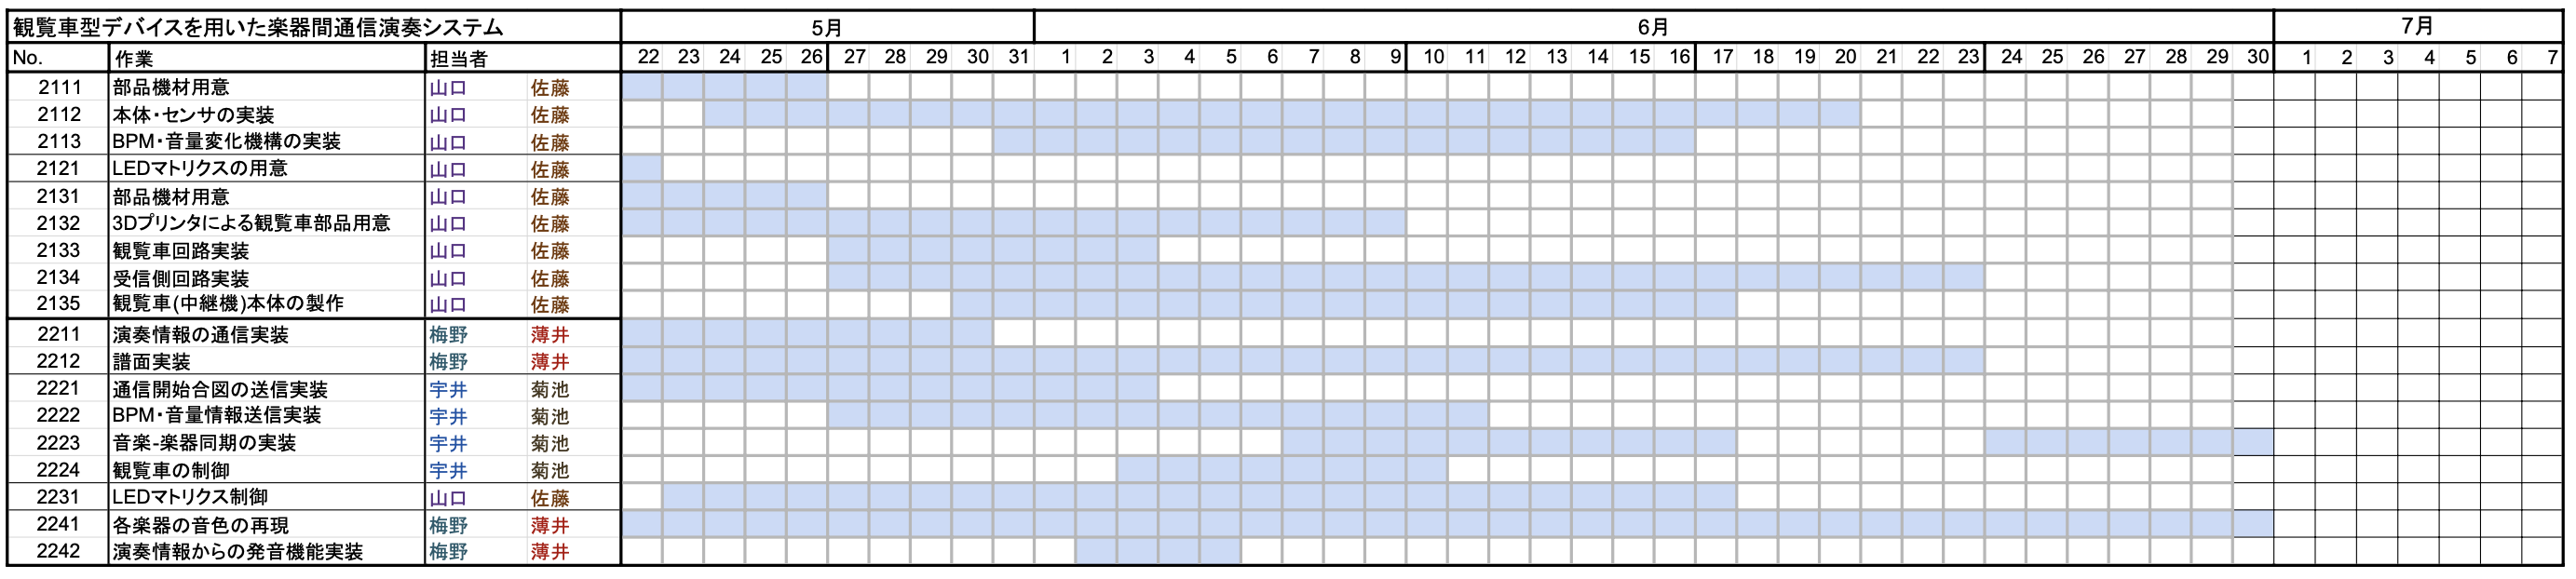
\includegraphics[width=0.9\columnwidth]{gant13.png}
    \caption{計画段階のガントチャート（実装フェーズ）}
    \label{fig:gant13}
\end{figure}

\begin{figure}[htbp]
    \centering
    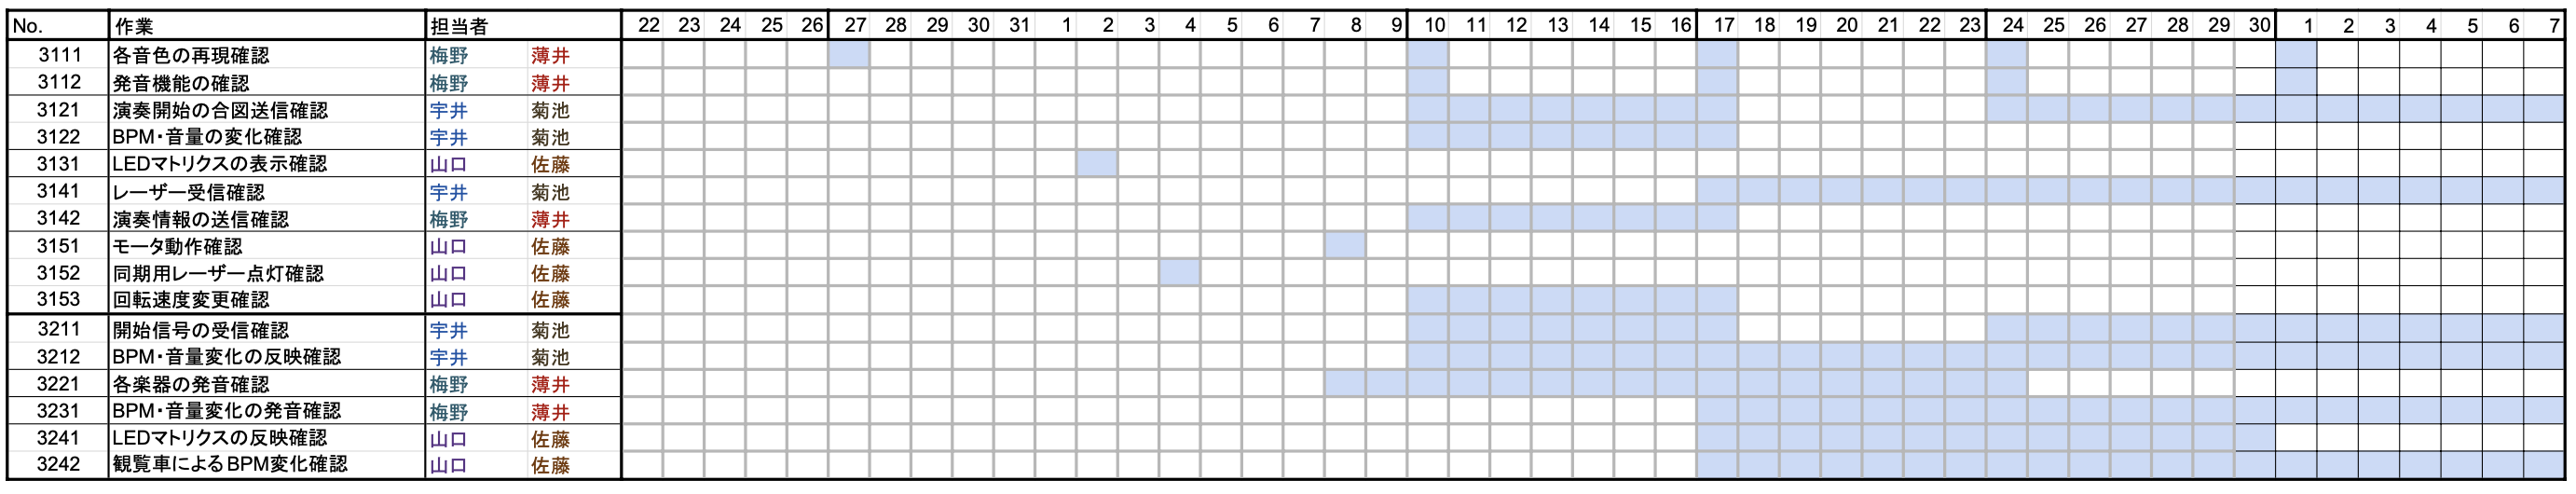
\includegraphics[width=0.9\columnwidth]{gant14.png}
    \caption{計画段階のガントチャート（テストフェーズ）}
    \label{fig:gant14}
\end{figure}

次に，現在のGCを図\ref{fig:gant15}に示す．達成した項目は緑色で塗られている．

\begin{figure}[htbp]
    \centering
    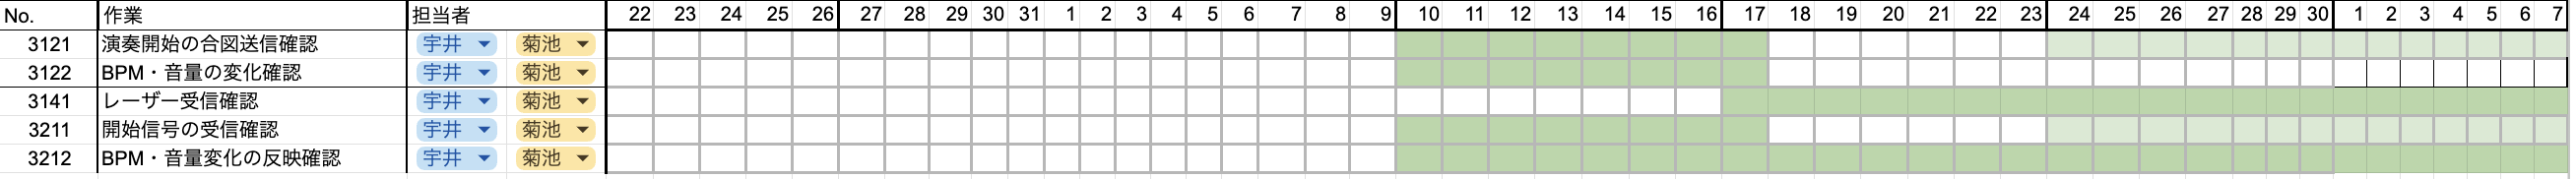
\includegraphics[width=0.9\columnwidth]{gant15.png}
    \caption{現在のガントチャート}
    \label{fig:gant15}
\end{figure}


\sectionrule


\section{AI利用状況と検証（再現性重視）}

今回はAIを利用していない．

\sectionrule


\section{次回計画}


\begin{itemize}

  \item 目標：最終発表に向けた準備
    \begin{itemize}
      \item 最終調整を行う．
      \item 発表資料の作成を進める．
    \end{itemize}

  \item 達成基準：
    \begin{itemize}
      \item 全テスト項目が完了し，システム全体が正常に動作すること．
    \end{itemize}

  \item 期限：
    \begin{itemize}
      \item 2026/7/14
    \end{itemize}

\end{itemize}


\sectionrule


\end{document}
